\documentclass[11pt]{beamer}

\RequirePackage{silence}
\WarningFilter{remreset}{The remreset package}

\usetheme{Copenhagen} %metropolis#
\useoutertheme{infolines}
\usecolortheme{default}

%%%%%%%%%%%%%%%%%%%%%%%%%%%%%%%%%%%%%%%%%%%%%%%%%%%%%%%%%%%%%%
%
% 1. Personendaten
%
\author[Diener, Roob, B{\'e}k{\'e}si]
{Irene~Diener, Toni~Roob, Jarod~A.~M.~B{\'e}k{\'e}si}
\newcommand{\myTitle}{Einf{\"u}hrung in die Quantenkommunikation}
\newcommand{\myTitleShort}{Quantenkommunikation}
\title[\myTitleShort]{\myTitle}
%\subtitle{}
\newcommand{\myProf}{Prof.~Dr.~habil.~Andriy~Luntovskyy}
\newcommand{\myAcademy}{Duale Hochschule Sachsen}
\newcommand{\myStudy}{Studiengang Informationstechnik}
\newcommand{\myLocation}{Dresden} 
\newcommand{\myVersion}{Version 1.0}
% Abgabedatum
\newcommand{\mySubmissionDate}{30. September 2025}


%%%%%%%%%%%%%%%%%%%%%%%%%%%%%%%%%%%%%%%%%%%%%%%%%%%%%%%%%%%%%%
%
% 2. Packete
%
\usepackage[latin1]{inputenc}
\usepackage[T1]{fontenc}
\usepackage{lmodern}

\usepackage{hyphenat}
\usepackage[ngerman,english]{babel}
\usepackage[babel]{csquotes}
\usepackage{cite}
\usepackage{amsmath,amssymb,amstext,amsthm}
\usepackage{upgreek,units}

\usepackage{ragged2e}
\usepackage{animate}

\usepackage{graphicx}
\usepackage{caption,subcaption}

\usepackage[hang,multiple]{footmisc}
\renewcommand{\footnotemargin}{1.2em}
\usepackage{longtable,booktabs,multirow,colortbl}
\usepackage{rotating}
\usepackage{remreset}

\usepackage{enumerate}
\usepackage[shortlabels]{enumitem}
\setlist{noitemsep, itemsep=3pt, topsep=0pt, partopsep=6pt}


%%%%%%%%%%%%%%%%%%%%%%%%%%%%%%%%%%%%%%%%%%%%%%%%%%%%%%%%%%%%%%
%
% 3. Settings
%
\date{\mySubmissionDate}

\logo{
\includegraphics[width=2cm]{figures/CD/DHSN-Logo}}
\setbeamercovered{transparent}


%The next block of commands puts the table of contents at the 
%beginning of each section and highlights the current section:
\AtBeginSection[]
{
	\begin{frame}[allowframebreaks]
		\frametitle{Inhaltsverzeichnis}
		\tableofcontents[currentsection]
	\end{frame}
}

%
% Sil-ben-tren-nung
%
\hyphenation{Do-nau-dampf-schiff-fahrt}

%
% Ab hier der eigentliche LaTeX-Satz
%
\begin{document}
	%\setbeamertemplate{navigation symbols}{}
	\begin{frame}
		\maketitle
	\end{frame}
	
	\begin{frame}
		\begin{tabular}{cc}
			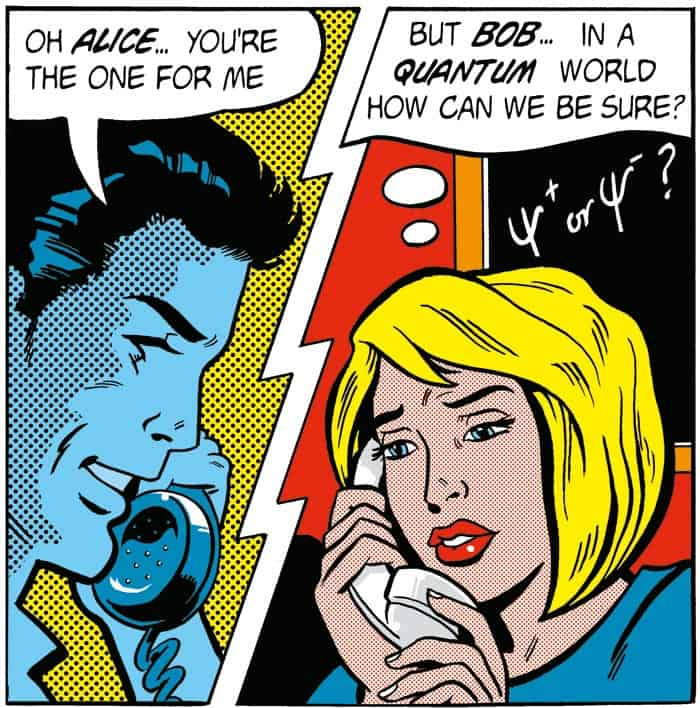
\includegraphics[scale=0.25]{figures/Communication-without-particles-pic1} &  \\
		\end{tabular}
	\end{frame}
	
	\section{Was ist Quantenkommunikation?}
\begin{frame}[allowframebreaks]
	\begin{theorem}
%		\justifying
		Quantenkommunikation ist die Nutzung der \enquote{Prinzipien der Quantenmechanik wie Quantenverschr{\"a}nkung und Quantensuperposition, um Informationen nahezu abh{\"o}rsicher zu {\"u}bertragen}.\cite{frauenhofer2025}
	\end{theorem}
\end{frame}
	\section{Was sind Quanten?}
\begin{frame}[allowframebreaks]

\end{frame}
	\section{Grundlagen der Quantenkommunikation}
\begin{frame}

\end{frame}
	\section{Grundlagen der Quantenmechanik}
\begin{frame}
	
\end{frame}
	\section{Quantenteleportation \& Quantennetzwerke}
\begin{frame}
	
\end{frame}
	%*************************************************************************
	% Literaturverzeichnis
	%*************************************************************************
	\section{Quellenverzeichnis}
	\begin{frame}[allowframebreaks]
		\frametitle{Quellenverzeichnis}
		\bibliographystyle{baalphadin}
		%		\pdfbookmark[-1]{Quellenverzeichnis}{pdf-Bibliography}%
		%		\phantomsection%
		% BibTeX:
		\bibliography{bibliography}
	\end{frame}
	
\end{document}